\section{Problem setting, network and data}\label{sec:setting}

\subsection{The fulfilment network}
We study a stylised but realistically dimensioned outbound network for mainland Spain and Portugal (\cref{fig:network}).
Demand originates in $|\J|=65$ \emph{zones}: the 47 mainland Spanish provinces and the 18 mainland Portuguese districts, located at their capitals and weighted by census population (53.9 million inhabitants in total).
Units are shipped from $|\I|=10$ fulfilment centres (FCs) located in well-known Iberian logistics hubs (two in Madrid, two in Barcelona, Zaragoza, Seville, Valencia, Asturias, Bilbao and Murcia), travel on scheduled line-haul trucks to one of $|\Hs|=12$ sort centres (SCs), and are delivered by the last mile to the customer zone.
A zone is served by the nearest SC of its own country, so the decision \emph{which FC ships a unit} also fixes its middle-mile lane $(i,h(j))$.
Products belong to $|\K|=4$ categories with different volume $v_k$ (truck package-equivalents per unit) and labour content $l_k$ (labour units per unit): small sortable ($v=1$, $l=1$), medium sortable ($2.2$, $1.4$), bulky non-sortable ($7$, $3$) and apparel ($1.3$, $0.9$).
Bulky items are only stocked in the four large non-sortable sites, which makes their assignment far less flexible.

\begin{figure}[t]
  \centering
  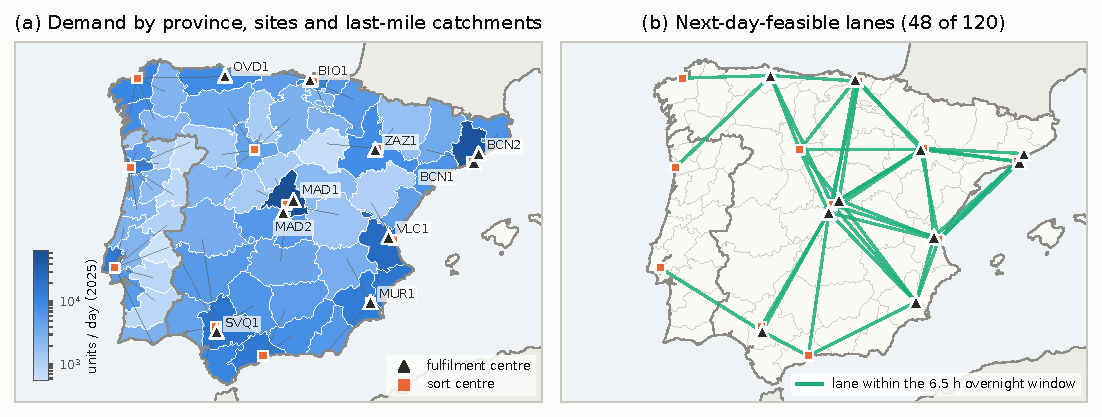
\includegraphics[width=\linewidth]{network}
  \caption{(a) The network on the Iberian Peninsula: provinces and districts shaded by mean daily demand (log scale), fulfilment centres (triangles), sort centres (squares) and the last-mile catchment of every sort centre (thin lines). (b) Lanes whose line-haul transit fits the overnight window, i.e.\ lanes that keep the next-day promise. Only 48 of the 120 lanes are next-day feasible, so where a unit ships from decides whether the promise is kept. Boundaries: Natural Earth (public domain).}
  \label{fig:network}
\end{figure}

\paragraph{Distances, transit times and the speed promise.}
Road distances are great-circle distances inflated by a circuity factor of $1.22$, which is typical for the Iberian road network.
A lane's transit time is $\text{km}/80 + 0.5$ hours (driving plus loading/unloading).
Trucks leave the FC after the evening cut-off and must reach the SC before the early-morning sort.
A unit is therefore delivered \emph{on time} (next day) if and only if its lane fits the $6.5$-hour overnight window, and \emph{late} (day $+2$) otherwise.
Only 48 of the 120 lanes are next-day feasible (\cref{fig:network}b); 23 zones (mostly Galicia, Portugal and Andalusia) can be served on time by exactly one FC, and 63\% of all FC--zone--category arcs are late.
This gives the cost--speed trade-off its bite: the cheapest FC with free capacity is often a late one.

\paragraph{Costs.} All monetary values are in euros per day; \cref{tab:params} lists every parameter.
A scheduled truck on lane $(i,h)$ costs $F_{ih} = 180 + 1.25\cdot\text{km}_{ih}$ (\EUR{181}--\EUR{1719}) and carries $Q=1400$ package-equivalents.
Capacity bought on the day from the spot/LTL market costs $1.8\times$ the scheduled rate per package-equivalent.
Labour is scheduled in crews of 10 associates for one shift ($\pi = 2000$ labour units for \EUR{1760}, i.e.\ \EUR{0.88} per labour unit).
Up to 30\% overtime can be added at a $1.6\times$ premium.
Each FC has a maximum number of crews and of outbound truck departures (dock slots).
Shipping a unit incurs an FC processing cost and a last-mile cost ($2.60 + 0.012$\,\EUR{}/km from the SC, \EUR{2.61}--\EUR{6.02}).
A unit that cannot be shipped today misses its promise and costs $p = \EUR{15}$ (re-handling, compensation and cancellation risk; \cref{sec:sensitivity} discusses this choice).
A late unit costs $\lambda = \EUR{1}$, the \emph{price of speed}; this weight is the dial of the multi-objective analysis in \cref{sec:pareto}.
CO$_2$ is accounted at $0.9$\,kg per truck-km, with a $1.35\times$ factor for less consolidated spot capacity.



\begin{table}[t]
\centering\small
\caption{Network and cost parameters (base case).}\label{tab:params}
\begin{tabular}{@{}lll@{}}
\toprule
Parameter & Value & Meaning \\ \midrule
$Q$ & 1400 pkg-eq & trailer capacity \\
$F_{ih}$ & $180 + 1.25\,\text{km}_{ih}$ & cost of a scheduled truck on lane $(i,h)$ \\
$s_{ih}$ & $1.8\,F_{ih}/Q$ & spot capacity cost per package-equivalent \\
$\pi$, $L$ & 2000 labour units, \EUR{1760} & capacity and cost of one crew-shift \\
$\rho$, $c^{\mathrm{ot}}$ & 0.30, $1.6\,L/\pi = \EUR{1.41}$ & overtime cap (fraction) and cost per labour unit \\
$W_i$, $D_i$ & 22--70 crews, 60--150 trucks & site limits (total 426 crews, 1020 departures) \\
$c^{\mathrm{fc}}_i$ & \EUR{0.24}--\EUR{0.31} & FC variable processing cost per unit \\
$c^{\mathrm{lm}}_j$ & $2.60 + 0.012\,\text{km}_{h(j),j}$ & last-mile cost per unit \\
$p$, $\lambda$ & \EUR{15}, \EUR{1} & penalty for an unshipped unit; price of a late unit \\
window & 6.5 h at 80 km/h + 0.5 h & overnight line-haul window \\
CO$_2$ & 0.9 kg/truck-km; 0.18 kg/unit last mile & emission factors \\ \bottomrule
\end{tabular}
\end{table}

\paragraph{Inventory.} Inventory placement is decided upstream on a longer horizon and is exogenous here.
For each day, FC $i$ holds $\mathrm{Inv}_{ik}$ units of category $k$: a national cover of $1.35$ days of expected demand, split across the FCs stocking $k$ in proportion to their size and distorted by a persistent log-normal imbalance (standard deviation 0.25).
Inventory is thus not perfectly aligned with demand, which is what makes the \emph{online} assignment problem (\cref{sec:online}) non-trivial.

\subsection{A generative demand model}\label{sec:dgp}
Real order data are proprietary, so we build a \emph{generative} data set.
This is a feature, not only a necessity: because the latent states are known, the \emph{true} conditional distribution of tomorrow's demand can be sampled exactly.
That provides an oracle forecaster, and it lets us measure the economic value of forecast quality without the noise of a single realised path (\cref{sec:value-forecast}).
Daily outbound units $y_{tjk}$ for day $t$, zone $j$ and category $k$ follow
\begin{align}
  y_{tjk} &\sim \mathrm{NegBin}\big(\text{mean } \mu_{tjk},\ \text{dispersion } r_k\big), \nonumber\\
  \log \mu_{tjk} &= \underbrace{\log b_{jk} + \tau_{tj} + \omega_k(\mathrm{dow}_t) + \alpha_{k,c(j)}(\mathrm{doy}_t)
     + e_{tk,c(j)} + \eta^{\mathrm{hol}}_{tj} + \phi_{tk} + \beta^\top_k z_{tj}}_{\text{known at forecast time: calendar, promotions, weather}} \nonumber\\
  &\quad + \underbrace{\eta_t + \xi_{t,r(j)} + \zeta_{tk}}_{\text{latent AR(1) shocks}} .
  \label{eq:dgp}
\end{align}
The terms are:
\begin{itemize}
  \item a base level proportional to population, with an urbanisation premium, a lower e-commerce penetration in Portugal ($0.72$) and zone-specific category mixes;
  \item log-linear growth of 10\% (Spain) and 16\% (Portugal) per year;
  \item category-specific weekly profiles (units to \emph{ship} peak on Monday, \cref{fig:demand}b);
  \item a smooth annual cycle with a pronounced August dip in Spain;
  \item retail events: Black Friday week and Cyber Monday with a multi-day shipping tail, two Prime events per year, the Christmas ramp and trough, the Spanish \emph{Reyes Magos} peak, the January \emph{rebajas} for apparel, and back-to-school;
  \item national and regional public holidays (including moving Easter holidays), with a catch-up effect the day after;
  \item announced flash promotions per category;
  \item weather covariates $z_{tj}$: spatially correlated temperature anomalies and rain, which raise online demand slightly; cold snaps lift apparel.
\end{itemize}
The unpredictable part consists of three AR(1) processes: a national shock $\eta_t$ (autocorrelation 0.8), regional shocks $\xi_{t,r}$ (0.6) and category shocks $\zeta_{tk}$ (0.7).
On top of these comes negative-binomial count noise, with dispersion between 45 (bulky) and 160 (small sortable).
The resulting series have a coefficient of variation of about 14\% at the zone--category level and 5\% for the national total.

The simulation covers January 2023 to December 2026.
Volume averages $443$ thousand units per day in 2025 and peaks at $1.17$ million on Prime Day 2026 (\cref{fig:demand}a); the scale is plausible for a large Iberian e-commerce network.

\begin{figure}[t]
  \centering
  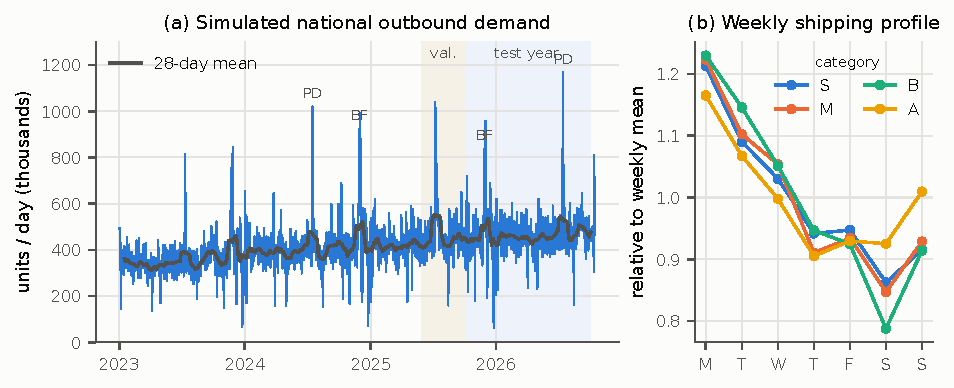
\includegraphics[width=\linewidth]{demand}
  \caption{(a) Simulated national daily units to ship; shaded: validation window and test year (BF: Black Friday, PD: Prime Day). (b) Weekly profile per category: orders placed at the weekend ship on Monday; apparel is flatter.}
  \label{fig:demand}
\end{figure}

\subsection{Decision hierarchy}
The study follows the decision hierarchy of an outbound fulfilment organisation:
\begin{enumerate}
  \item \textbf{Forecasting} (\cref{sec:forecasting}): every evening, probabilistic forecasts of next-week demand per zone and category, and joint scenarios for the next day.
  \item \textbf{Day-ahead capacity planning} (\cref{sec:planning}--\cref{sec:pareto}): commit the number of scheduled trucks per lane and labour crews per FC before demand is known, anticipating that the order assignment will adapt to realised demand.
  \item \textbf{Online order assignment} (\cref{sec:online}): during the day, assign each arriving unit to an FC irrevocably, consuming the committed capacity.
  \item \textbf{Strategic what-if} (\cref{sec:network}): evaluate a network investment with the same machinery.
\end{enumerate}
